\chapter{Muestras y Procedimientos}

\label{ch:samples-procedure}

En este capítulo se describen las muestras simulada y observada, el método de interpretación de
$\set{\sedt[F]{obs}}$ y los procedimientos para el análisis de los resultados.

%----------------------------------------------------------------------------------------

\section{Los sondeos relevantes}

Ya que la resolución espectral de las observaciones es una cantidad que varía de un sondeo a otro,
es un parámetro sensible para evaluar del contenido estelar que se puede extraer de los sondeos de
galaxias como función de éste. En ese sentido se ha planteado hacer dicha evaluación a tres
resoluciones espectrales distintas: fotometría de banda ancha, de banda angosta y espectroscopía de
alta resolución. Para contextualizar el análisis en el marco de sondeos reales se han escogido el
\emph{Sloan Digital Sky Survey} \citep[SDSS,][]{York2000}, que proporcionará la información para
construir las muestras espectroscópica \citep{Strauss2002} y fotométrica de banda ancha
\citep{Gunn1998} y, el \emph{Javalambre Physics of the Accelerating Universe Astrophysical Survey}
\citep[J-PAS,][]{Benitez2014,Dupke2015} que proporcionará la información para construir la muestra
fotométrica de banda angosta. Este último sondeo será de particular interés a lo largo de este
trabajo puesto que promete superar la información provista por otros sondeos en la recuperación de
la abundancia química estelar en las galaxias, un parámetro físico que ha permanecido elusivo hasta
ahora en sondeos fotométricos tradicionales \citep[aún así véase,][]{MacArthur2010}.

\subsection{La muestra simulada}\label{sc:mock-sample}

\begin{SCfigure}
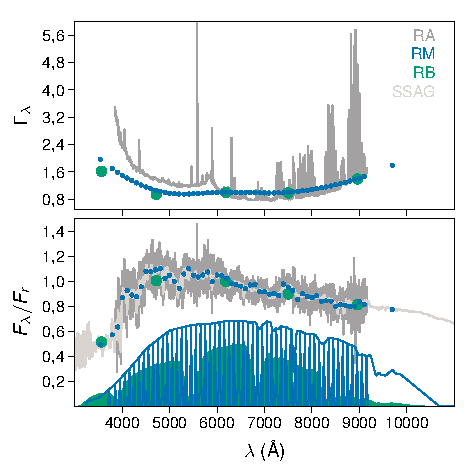
\includegraphics{figures/sigma-spectrum}
%
\caption{\emph{Arriba:} Distribución espectral del ruido instrumental típico a las diferentes
resoluciones: espectroscopía del SDSS (RA: \emph{gris}), fotometría del J-PAS (RM: \emph{azul}) y
del SDSS (RB: \emph{verde}). Se muestra un espectro ejemplo a las resoluciones espectrales
correspondientes. \emph{Abajo:} Como ejemplo se muestra la misma DEE ``observada'' por los distintos
instrumentos, junto con la original (SSAG: \emph{en gris claro}). La función de transmisión de las
cámaras fotométricas del J-PAS y del SDSS tomando en cuenta la contribución de la atmósfera
terrestre también se muestran.}
%
\label{fig:sigma-spectrum}
\end{SCfigure}

\citet{Chen2012} introdujeron una receta para simular observaciones de galaxias usando un método de
Monte Carlo para muestrear el espacio de parámetros de funciones las $\zeta(Z_0,t)$ y $\psi(Z;t)$
previamente definidas por los autores. \citet{Magris2015} implementaron esta receta en una
biblioteca llamada \emph{Synthetic Spectral Atlas of Galaxies} (SSAG) para probar varias
implementaciones del método de la síntesis espectral. En el presente trabajo se utilizará la misma
muestra de $134$ HFEs usadas en \citet{Magris2015}.

Los espectros de la SSAG, por construcción, tienen un muestreo espectral
$\Delta\lambda=\unit[1]{\AA}$. Entonces, a partir de estos espectros se sintetizarán la
espectroscopía del SDSS caracterizada por una Resolución Alta \citep[RA:
$\Delta\lambda=1\,\text{\AA}$][]{Strauss2002}, y la fotometría del J-PAS de Resolución Media
\citep[RM: $\Delta\lambda=140\,\text{\AA}$][]{Marin-Franch2015} y la fotometría del SDSS de
Resolución Baja \citep[RB: $\Delta\lambda\sim1000\,{\AA}$][]{Doi2010}, ambas usando la integral del
flujo esperado en la $k$-ésima banda espectral:
%
\begin{equation}\label{ec:flujo-esperado}
F_k = \left.\int T_k(\lambda)\,f_\lambda\,\text{d}\lambda\middle/\int T_k(\lambda)\,\text{d}\lambda\right.,
\end{equation}
%
donde las funciones de respuesta, $T_k(\lambda)$, de ambos sistemas fotométricos son como se muestra
en la Fig.~\ref{fig:sigma-spectrum}. Aunque la SSAG por sí misma no proporciona distribuciones de
índices espectrales realistas, pues los fenómenos físicos que regulan el contenido estelar no entran
en la simulación, la muestra sintética se ha escogido de manera que la bimodalidad en las
distribuciones de propiedades observacionales como el color y la discontinuidad de
$\unit[4000]{\AA}$ estén presentes como en sondeos reales \citep{Strateva2001, Kauffmann2003,
Baldry2004}.

Para simular datos espectrales realistas a las distintas resoluciones espectrales, se procederá como
sigue: \textit{(i)} se añadirá ruido Gaussiano aleatoriamente al flujo en cada elemento de
resolución asumiendo ruido no correlado, lo cual es observacionalmente plausible. Para esto se
construye una función $\Gamma_\lambda$ tal que ésta es el promedio de los errores reportados por el
SDSS en la espectroscopía de galaxias hasta $z=0.1$, normalizado a la unidad en la longitud de onda
efectiva de la banda $r'$ \citep{Magris2015}. Dicha función será luego suavizada y degradada en
resolución para ajustarse a las distintas resoluciones espectrales estudiadas en este trabajo. En la
Fig.~\ref{fig:sigma-spectrum} se muestran las curvas $\Gamma_\lambda$ resultantes. En este sentido,
el espectro ``observado'' resultante será simplemente:
%
\begin{equation}\label{ec:noise-flux}
\sedt[F]{obs} = {F_\lambda} + \mathcal{N}(\mu,\sigma_\lambda),
\end{equation}
%
donde $\mathcal{N}(\mu,\sigma_\lambda)$ representa una realización aleatoria de una distribución
Gaussiana con promedio $\mu=0$ y desviación estándar $\sigma_\lambda=\Gamma_\lambda
F_\lambda/(S/N)_r$ en cada elemento de resolución espectral. Para tomar en consideración el hecho de
que la relación señal a ruido es $S/N\propto
\left.\sedt[F]{obs}\middle/\sqrt{\sedt[F]{obs}+\sigma_\text{ins}}\right.$, donde $\sigma_\text{ins}$
es la desviación estándar del ruido introducido por el instrumento, se adoptará distintos valores de
ésta en la banda $r'$, $(S/N)_r=20$, $45$ y $140$ para los datos a RA, RM y RB, respectivamente.
Nótese que estos valores son consistentes con las expectativas para sondeos reales de galaxias en el
Universo local \citep{Benitez2014, Howell2006}. Para tomar en consideración las variaciones
estadísticas de los parámetros físicos recuperados como función del ruido observacional, el
procedimiento de añadir el ruido aleatorio se repetirá $20$ veces para cada espectro en la muestra
de $134$ galaxias, de manera que la muestra final comprenderá $2680$ espectros en tres resoluciones
espectrales, representativos de las observaciones reales en el Universo local. El resultado de una
de las realizaciones de ruido se muestra en una proyección del espacio de colores del SDSS en la
Fig.~\ref{fig:samples} en azul oscuro.

Es importante notar que el número de realizaciones que se adoptará es completamente arbitrario y
representa un compromiso entre un tiempo de cómputo razonable y resultados estadísticamente
robustos. A lo sumo se espera que este número de realizaciones permitirá un estudio espectro por
espectro ($2680$) y no HFE por HFE ($134$) debido a la variabilidad esperada en parámetros físicos
como la edad y la metalicidad \citep[\eg,][]{Magris2015}.

\subsection{La muestra observada}\label{sc:obs-sample}
\begin{SCfigure}
\centering
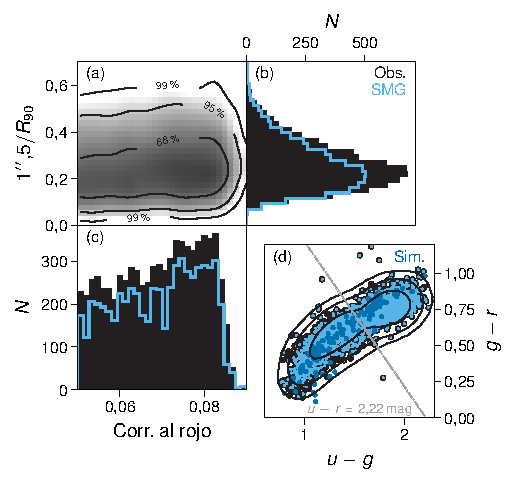
\includegraphics[scale=1]{figures/sample_chars}
%
\caption{\emph{(a)} La fracción de luz muestreada por la fibra de $\unit[1.5]{arcseg}$ con respecto
del radio Petrosiano al $\unit[90]{por ciento}$ de la luz ($\unit[1.5]{arcseg}/R_{90}$) como función
del corrimiento al rojo cosmológico para la muestra de galaxias observadas (\cf,
\S\ref{sc:obs-sample}). \emph{(b)} La distribución marginal correspondiente al eje de las ordenadas
y, \emph{(c)} la correspondiente al eje de las abscisas \emph{(negro)}. \emph{(d)} El diagrama $g-r$
\emph{versus} $u-g$ para la muestra observada \emph{(negro)} con los correspondientes contornos de
confiabilidad a $1$, $2$ y $3\,\sigma$. En el mismo plano se muestran la Submuestra de Garching
(SMG; \emph{azul claro}) y la muestra de galaxias sintéticas \emph{(azul oscuro)}. El separador
entre GFE y GPa también se muestra \emph{(línea a trazos)}.}
%
\label{fig:samples}
\end{SCfigure}

Para construir la muestra observada, se seleccionará un conjunto de $\sim\unit[7]{k}$ espectros de
galaxias de las observaciones espectroscópicas del SDSS-DR7 \citep{Abazajian2009}, con las
siguientes restricciones: \textit{(i)} la relación señal a ruido debe ser $>10$ para minimizar el
impacto de las degeneraciones en los parámetros físicos recuperados; \textit{(ii)} las galaxias
deben estar en el universo local, $z\leq0.09$, de manera que los espectros representan observaciones
en el rango óptico; y \textit{(iii)} el número de pixeles buenos debe ser superior a $3850$.
Adicionalmente, aquellas regiones del espectro donde se manifiestan las líneas de emisión
[O\textsc{ii}]$\lambda\lambda3726,3729$, H$\gamma$, H$\beta$,
[O\textsc{iii}]$\lambda\lambda4959,5007$, He\textsc{i}$\lambda5876$, [O\textsc{i}]$\lambda6300$,
[N\textsc{ii}]$\lambda\lambda6548,6583$, H$\alpha$, y [S\textsc{ii}]$\lambda\lambda6717,6731$ serán
enmascaradas (removidas) dentro de $\approx\unit[20]{\AA}$, sin importar si están presentes o no.
Para facilitar el análisis en términos del contenido estelar (población vieja y población jóven), la
muestra resultante se dividirá en Galaxias con Formación Estelar (GFE, $u-r<\unit[2.22]{mag}$) y en
Galaxias Pasivas (GPa, $u-r\geq\unit[2.22]{mag}$) de acuerdo con \citet{Strateva2001}. En la
Fig.~\ref{fig:samples}\textit{d} se muestra en la región en escala de grises el mapa de densidad de
la muestra observada en el plano $g-r$ \emph{versus} $u-g$, los contornos representan las regiones
de confianza de $1$, $2$ y $3\sigma$. Un subconjunto de galaxias de la muestra observada fue
estudiado por \citet{Gallazzi2005}. Para anclar los resultados presentados en este trabajo con los
disponibles en la literatura, se usará los resultados de \citet{Gallazzi2005} para este subconjunto
el cual será referido en adelante como Submuestra de Garching (SMG)\footnote{disponible en la red en
\url{http://www.mpa-garching.mpg.de/SDSS/}.}. En la Fig.~\ref{fig:samples} la SMG es representada en
azul claro.

Ya que los datos fotométricos del J-PAS no existen aún, para probar la consistencia entre los
parámetros derivados a partir de la espectroscopía de RA y los derivados a partir de la fotometría
de RM, se sintetizará observaciones a esta última resolución espectral a partir de las observaciones
espectroscópicas del SDSS. Para esto se calculará el flujo esperado a través de la cámara
fotométrica del J-PAS,  usando la integral en la Ec.~\eqref{ec:flujo-esperado}, donde $f_\lambda$
será sustituido por el espectro en reposo de cada galaxia y $T_k(\lambda)$ por la función de
respuesta de la cámara del J-PAS en el $k$-ésimo filtro \citep{Marin-Franch2015}. Una medida del
error en $F_k$ es proporcionada por la propagación de errores convencional
\citep[\eg,][]{Bevington2003} usando la relación
%
\begin{equation}\label{ec:error-prop}
\sigma_k^2 = \int_\lambda T_k(\lambda)^2\sigma_\lambda^2\text{d}\lambda,
\end{equation}
%
donde $\sigma_\lambda$ es la desviación estándar en la medida $f_\lambda$ reportada por el
SDSS.

Los espectrógrafos del SDSS están configurados para cubrir la región espectral
$3800\,$---$\,\unit[9200]{\AA}$ \citep{Strauss2002}, mientras que la cámara del J-PAS comprenderá el
rango $\sim3500\,$---$\,\unit[10000]{\AA}$ \citep{Marin-Franch2015}. De manera que alrededor de
cinco elementos de resolución del J-PAS no estarán presentes. Más aún, aquellas regiones de los
espectros del SDSS donde más del $10$ por ciento de los pixeles dentro de una banda fotométrica del
J-PAS hayan sido reportados como píxeles malos, se traducirá en que la banda correspondiente será
removida del espectro sintetizado. Así que alrededor de $10$ medidas del flujo a la resolución de
J-PAS serán enmascaradas de los espectros sintetizados. Entonces, de la configuración original de
$56$ medidas del flujo planeada para J-PAS, solo unas $\sim40$ medidas serían representadas en la
muestra sintética en el mejor de los casos, \ie, sin tomar en cuenta las regiones enmascaradas para
remover el efecto de la emisión del gas en el MIE. Por esta razón, para mitigar las consecuencias
que esta incompletitud de información en los espectros sintéticos podría tener en el análisis de los
resultados, el procedimiento para remover el efecto de la emisión del gas se realizará \emph{a
posteriori}, es decir, después de sintetizar los espectros J-PAS, de manera que \emph{solo} los
elementos de resolución afectados por dicha emisión serán removidos. Así, los espectros sintéticos
tendrán alrededor de $\sim40$ elementos de resolución. Finalmente, para establecer una diferencia
entre las DEE de la muestra observada a una resolución y sus correspondientes contrapartidas
simuladas, debido a los artefactos antes mencionados (\eg, remoción de las líneas de Balmer y
píxeles malos), las DEE observadas a RA y RM serán referidas como RA\up{*} y RM\up{*},
respectivamente.

%----------------------------------------------------------------------------------------

\section{El método}

El método de síntesis espectral, ajuste espectral o síntesis inversa ha sido rutinariamente
utilizado para extraer el contenido estelar de las galaxias no resueltas desde que aparecieron
públicamente los primeros sondeos de galaxias con el suficiente poder estadístico. Estos métodos
pueden dividirse en dos clases, dependiendo de las suposiciones que se hacen sobre las funciones
$\zeta(Z_0,t)$ y $\psi(Z;t)$. Por una parte está el método paramétrico que, como su nombre indica,
consiste en parametrizar dichas funciones bajo un conjunto de suposiciones físicamente plausibles
\citep[\eg,][]{Kauffmann2003, Brinchmann2004, Gallazzi2005, Kriek2009}. Bajo este esquema, los
parámetros definitorios de $\zeta(Z_0,t)$ y $\psi(Z;t)$ de entrada se suponen inciertos, de manera
que pueden ser descritos por distribuciones de probabilidad que reflejan el conocimiento
\emph{previo} sobre los fenómenos físicos involucrados. Así, la extracción del contenido estelar de
las observaciones se implementa naturalmente en el marco de la inferencia estadística, generalmente
usando el Teorema de Bayes \citep[véase apéndice en][]{Kauffmann2003}. Por otro lado, el método no
paramétrico no supone una forma funcional fija para $\zeta(Z_0,t)$ y $\psi(Z;t)$ más allá de las
restricciones necesarias en el muestreo de las variables $t$ y $Z$. Esta flexibilidad del método no
paramétrico será particularmente explotada en este trabajo y se explicará en más detalle a
continuación.

\subsection{Ajuste espectral no paramétrico}

El problema planteado por el método no paramétrico de ajuste espectral consiste en modelar la DEE
observada $\sedt[F]{obs}$ a partir de la función de verosimilitud $\lik{\sedt[F]{obs}}{\hip}$ que,
bajo la suposición generalmente plausible de que las incertidumbres en los datos son Gaussianas y no
están correlacionadas entre sí, es simplemente:
%
\begin{equation}\label{ec:likelihood}
\lik{\sedt[F]{obs}}{\hip} = \prod_{\lambda}^{\Ni{\lambda}}\frac{1}{\sqrt{2\pi{\sigma_\lambda}^2}}\exp{\left\{-\frac{\left[\sedt[F]{obs}-\sedt[F]{mod}(\hip)\right]^2}{2{\sigma_\lambda}^2}\right\}}
\end{equation}
%
donde $\sigma_\lambda$ es la desviación estándar en las medidas $\sedt[F]{obs}$. Este problema es
usualmente resuelto en el marco de la técnica de Máxima Verosimilitud o Máxima Probabilidad \emph{a
posteriori} \citep[\eg,][]{Heavens2000, CidFernandes2005}, que consiste en encontrar $\hhi$ tal que
$\lik{\sedt[F]{obs}}{\hhi}$ es máxima o, equivalentemente, encontrar el mínimo de la función de
mérito
%
\begin{equation}\label{ec:chi-square}
-2\log{\mathcal{L}}+\text{const}\equiv\chi^2(\hip) = \sum_\lambda^{\Ni{\lambda}}\frac{\left[\sedt[F]{obs}-\sedt[F]{mod}(\hip)\right]^2}{{\sigma_\lambda}^2}.
\end{equation}
%
Además, si el modelo propuesto es de la forma
%
\begin{equation}\label{ec:non-model}
\sedt{mod}(\hip) = \sum_{k=1}^{\Nt{PESs}}w^k(\hip)\sedi{k}(\hip),
\end{equation}
%
y los pesos $w^k(\hip)$ son lineales en $\hip$,\footnote{En esta notación la linealidad de
$w^k({\hip})$ está asegurada, pues los fenómenos físicos no lineales como la cinemática estelar y la
extinción por polvo se ya han sido capturados en $\sedi[F]{k}(\hip)$.} entonces $\chi^2(\hip)$ es
una función cuadrática del vector de parámetros y el problema se reduce a la resolución de un
sistema de $\Ni{\lambda}$ ecuaciones lineales con $\Nt{PESs}$ incógnitas.

\subsection{El algoritmo \emph{\dynbas}}

\emph{Dynamical Basis Selection} \citep[\dynbas;][]{Mateu2009, Mateu2010, Magris2015} es un
algoritmo no paramétrico de ajuste espectral diseñado para recuperar el contenido estelar de las
galaxias minimizando los efectos de degeneración intrínsecos del problema. La DEE es reconstruída
usando el modelo en la Ec.~\eqref{ec:non-model}, con
%
\begin{subequations}\label{ec:dyn-model}
\begin{align}
w^k(\hip) &= a_{ij}^k, \\
\sedi{k}(\hip) &= \sedi{k}(t_i, Z_j),
\end{align}
\end{subequations}
%
donde $i=1,\ldots,\Nt{edad}$ y $j=1,\ldots,\Nt{metalicidad}$. El algoritmo \dynbas por diseño usa un
número mínimo de ingredientes físicos (combinando hasta $\Nt{PESs}=3$ Poblaciones Estelares Simples,
PES) dinámicamente seleccionados para reproducir los rasgos del espectro problema, mediante la
consecución del mínimo absoluto de la función de mérito en Ec.~\eqref{ec:chi-square}, que se
encuentre en la región del espacio de parámetros muestreada durante el ajuste. Ya sea que el modelo
en las Ecs.~(\ref{ec:non-model} y \ref{ec:dyn-model}) sea ensamblado usando $\Nt{PESs}=1$, $2$ o $3$
componentes, dependerá de las peculiaridades de $\sedt[F]{obs}$.

Claramente \dynbas no está diseñado para recuperar la HFE en su máxima resolución temporal, sino
para hacer estimaciones robustas de las propiedades físicas globales, basadas en los rasgos más
importantes en la HFE de la galaxia problema. La implementación actual de \dynbas es factible para
la extracción del contenido estelar a partir de la DEE integrada de poblaciones estelares con HFE
relativamente simple \citep{Cabrera-Ziri2016}. A escalas extragalácticas la premisa se mantiene
\citep[\eg,][]{Diaz2015, Mejia-Narvaez2017}. \citet{Diaz2015} presentaron una implementación del
método no paramétrico llamada \textsc{muffit} en la que se seleccionan dinámicamente dos PES que en
combinación lineal son capaces de reproducir los rasgos espectrales más relevantes de las galaxias
de la secuencia roja (dominadas por poblaciones estelares viejas y ricas en metales evolucionando
pasivamente) a la resolución de la fotometría de ALHAMBRA \citep{Moles2008}. Independientemente,
usando simulaciones de observaciones espectroscópicas de galaxias con $S/N=20$, \citet{Magris2015}
compararon el desempeño de \dynbas frente a otros algoritmos de base fija y encontró que éste
recupera las propiedades físicas globales con una exactitud y precisión comparable con los
resultados de implementaciones que efectivamente buscan extraer la HFE (\eg, \starlight). Estos
resultados sugieren que las galaxias que resultan de HFE complejas pueden efectivamente ser
descritas por una combinación de las contribuciones espectrales de una población joven, intermedia y
una vieja \citep{CidFernandes2005}.

%----------------------------------------------------------------------------------------

\section{Los ingredientes y los parámetros físicos}

En este estudio se adoptará una versión actualizada de los modelos de síntesis de poblaciones
estelares de \defcitetalias{Bruzual2003}, basada en las trayectorias evolutivas de Padova 1994
\citep{Alongi1993, Bressan1993, Fagotto1994a, Fagotto1994b, Girardi1996} y bibliotecas de atmósferas
estelares actualizadas, denominadas \textsc{xmiless} para indicar el uso de una versión extendida de
las bibliotecas empíricas \miles{}$+$\stelib \citep{SanchezBlazquez2006, LeBorgne2003}. Se adoptará
la Función Inicial de Masa (FIM) de \citet{Chabrier2003} y se supondrá universalidad, \ie la FIM no
introducirá parámetros libres durante la interpretación de $\set{\sedt{obs}}$. En adelante a los
modelos así definidos se les llamará \bc{xm} para distinguirlos de los modelos originales de \bc.

\subsection{Los efectos del MIE}

Para asegurar la ventaja de la linealidad del problema no paramétrico, los fenómenos no lineales
serán tratados como se describe a continuación. Los modelos de síntesis de poblaciones estelares
escogidos para el presente estudio no incluyen emisión del gas, de manera que para hacerlo sería
necesario adoptar un modelo \citep[\eg,][]{Charlot2001} que introduciría más parámetros libres y,
probablemente más degeneraciones. En vista de que se ha restringido el presente estudio al contenido
estelar de las galaxias, la emisión del MIE ($L_{\lambda,\text{MIE}^+}$ en la
Ec.~\ref{ec:luminosidad-integrada}) no será modelada. En primer lugar, la muestra simulada descrita
en \S\ref{sc:mock-sample} fue construida usando los mismos modelos, entonces el conjunto de
``medidas'' $\set{\sedt[F]{obs}}$ será autoconsistente con la suposición en el modelo de que las
galaxias no presentan emisión del gas. Por otra parte, en el caso de la muestra observada, la
emisión del gas en las regiones de formación estelar (\eg, en GFEs), que será removida de las DEEs
como se describe en \S\ref{sc:obs-sample}, supondrá que la DEE resultante está en el mismo sistema
de los modelos sin emisión del gas, $\set{\sedt[F]{mod}}$.\footnote{Una última consideración sería
la emisión del polvo caliente en el MIE. Sin embargo, como la emisión del polvo es importante solo
en la región del infrarrojo del espectro, la restricción del presente estudio al rango óptico del
espectro será suficiente para despreciar este efecto en la construcción de $\set{\sedt[F]{mod}}$.}

La absorción/dispersión del MIE ($L_{\lambda,\text{MIE}^-}$ en la
Ec.~\ref{ec:luminosidad-integrada}), cuyo efecto neto es remover fotones de la línea de visión de la
galaxia observada, será introducido en $\set{\sedt[F]{mod}}$ usando una curva de extinción de la
forma $S_\lambda(\tauv)$. Físicamente se espera que la profundidad óptica, $\tauv$, sea una función
del tiempo ya que las regiones de formación estelar, donde el MIE se condensa lo suficiente como
para que la formación de granos de polvo ocurra \citep{Draine2009}, tienen un tiempo de vida del
orden de unas pocas decenas de millones de años \citep[véase,][para una revisión]{Lada2003}. El
modelo de extinción en dos fases de \citet{Charlot2000} intenta capturar esta física de la siguiente
manera: en la primera fase ($t_\star\leq\unit[10^7]{años}$) las estrellas se encuentran embebidas en
la nube molecular en que se formaron, la cual está caracterizada por una profundidad óptica $\tauv$
y, en la segunda fase ($t_\star>\unit[10^7]{años}$), solo una fracción $\mu$ de la profundidad
óptica original contribuye a la extinción en el MIE debido a la disociación de la nube molecular.
Así, el modelo de polvo en la muestra simulada estará caracterizado por dos curvas de extinción
[$S(\tauv)$ y $S(\mu\tauv)$], mientras que la muestra observada estará probablemente caracterizada
por fenómenos más complejos que los descritos por el modelo de \citet{Charlot2000}.
\citet{Tojeiro2007} demostraron que debido a las degeneraciones intrínsecas del problema de síntesis
espectral, no es posible recuperar ambos parámetros del polvo ($\tauv$ y $\mu$) de manera
simultánea. Por esta razón, en este estudio se buscará la recuperación de la extinción
\emph{efectiva}, que en el caso de las galaxias de la muestra sintética sería equivalente a estimar
$\tauv^\text{ef}\equiv\mu\tauv$, donde el parámetro libre, $\tauv^\text{ef}$, es la profundidad
óptica en la banda $V$ del MIE que está relacionada con la extinctión total en la banda $V$ mediante
$A_V\approx1.086\tauv^\text{ef}$. La mejor determinación del parámetro $A_V$ será buscada en el
rango plausible $0.0\,$---$\,\unit[1.5]{mag}$, de manera iterativa para asegurar un mínimo global de
la función $\chi^2(\hip)$ en la Ec.~\eqref{ec:chi-square}. En este trabajo se adoptará la curva de
extinción de \citet{Charlot2000} para modelar la muestra simulada de la SSAG (descrita en
\S\ref{sc:mock-sample}), siendo consistente con la SSAG, y la curva de \citet{Cardelli1989} con
$R_V=3.1$ para modelar la DEE de las galaxias en la muestra observada (descrita en
\S\ref{sc:obs-sample}).

\subsection{La cinemática estelar}

Si $\sedt[F]{obs}$ representa una observación espectroscópica ($\Delta\lambda\sim\unit[1]{\AA}$), la
cinemática estelar producirá un efecto notable ($\sim\unit[10]{\AA}$) en las líneas espectrales: la
rotación de las estrellas alrededor del centro de gravedad de la galaxia proyectada en la línea de
visión, produce un desplazamiento Doppler en el espectro observado cuyo efecto neto es el
ensanchamiento de las líneas de emisión/absorción. Para modelar este fenómeno, el conjunto de
observaciones $\set{\sedt[F]{mod}}$ será convolucionado con un \emph{kernel} Gaussiano,
$G(0,\sigma_v)$, donde $\sigma_v$ será la dispersión del campo de velocidades estelares estimada
para la galaxia. El mejor ajuste de $\sigma_v$ será buscado en el rango plausible
$0\,$---$\,\unit[400]{km\,s\up{-1}}$ de manera iterativa, ajustando una región angosta de
$\unit[100]{\AA}$ alrededor del rasgo espectral $\Caii$ H y K. En el caso de observaciones
fotométricas ($\Delta\lambda>\unit[100]{\AA}$), el efecto de la cinemática estelar será despreciable
y por lo tanto no será incluido en el modelo.

\subsection{El contenido estelar}

El contenido estelar de cada galaxia modelada es encapsulado por el algoritmo \dynbas en las tres
ternas $\set{a^k}$, $\set{t^k}$ y $\set{Z^k}$, donde se han omitido los índices $i$ y $j$ para
simplificar la notación. Aunque en principio estas ternas proporcionan la información para hacer una
construcción de las funciones $\zeta(Z_0,t)$ y $\psi(Z;t)$, dicha construcción a lo sumo ofrecerá
información sobre los eventos más relevantes (en términos de las medidas $\set{\sedt[F]{obs}}$) en
la historia de la galaxia problema hasta el instante $t_\text{emi}$ cuya unicidad, como ya se ha
mencionado antes, no está asegurada. Por esta razón muchos autores \citep[\eg,][]{Heavens2000,
Brinchmann2004, Gallazzi2005, Lee2009, CidFernandes2013, Magris2015} optan por reducir sus versiones
de la HFE y la HEQ (en la mayoría de los casos con muestreos más finos que $k\leq3$) usando alguna
estadística que represente estimados \emph{globales} del contenido estelar. En este trabajo se
procederá de la misma forma, como se describe a continuación.

La terna $\set{a^k}$ está directamente relacionada con la masa estelar, pues de entrada la DEE de
los modelos de PES de \bc{xm} está normalizada a una masa solar, luego, la luminosidad está
expresada en unidades de $\unit{\xsun{L}\,\AA\up{-1}\,\xsun{M}\up{-1}}$. Si además $\sedt[F]{obs}$
está expresado en unidades de $\unit{\xsun{L}\,\AA\up{-1}}$, los coeficientes $\set{a^k}$ serán
precisamente la contribución en masa (en unidades $\xsun{M}$) de gas en el MIE con metalicidad
$\set{Z^k}$ transformada en estrellas que en el instante $t_\text{emi}$ tenían una edad $\set{t^k}$.
Por otra parte, se adoptará la media ponderada por la masa estelar y ponderada por la luminosidad,
denotadas por $\mw{x}$ y $\lw{x}$, respectivamente, como estimados globales de la propiedad $x$
($=\log{t/\text{año}}$ o $\log{Z/\xsun{Z}}$) del contenido estelar en la galaxia problema. Estas se
definen como:
%
\begin{subequations}
\begin{align}
\mw{x} &= \frac{1}{M_\star}\sum_k^{\Nt{PESs}}a^k x_k, \\
\lw{x} &= \frac{1}{L_{\star,T}}\sum_k^{\Nt{PESs}}a^k L_T^k x_k,
\end{align}
\end{subequations}
%
donde los pesos cumplen las igualdades:
%
\begin{subequations}
\begin{align}
M_\star     &= \sum_k^{\Nt{PESs}}a^k, \\
L_{\star,T} &= \sum_k^{\Nt{PESs}}a^k L_T^k,
\end{align}
\end{subequations}
%
son la masa estelar total en la galaxia modelo y la luminosidad total calculada de acuerdo con la
Ec.~\eqref{ec:flujo-esperado} en una banda fotométrica cuya función de respuesta es $T_\lambda$. En
este trabajo se adoptará la luminosidad en la banda $r'$ del SDSS por poseer los errores de medición
mejor comportados en este sondeo. En general, $\lw{x}$ estará naturalmente sesgada hacia la
propiedad $x$ de la población estelar más luminosa en la región espectral muestreada por la banda
$r'$, mientras que la estimación $\mw{x}$ estará naturalmente sesgada hacia la propiedad del evento
de formación estelar más masivo ocurrido en la galaxia.

A continuación se describe el procedimiento para cuantificar la robustez de los parámetros
recuperados por \dynbas.

%----------------------------------------------------------------------------------------

\section{El tratamiento estadístico}

\subsection{Análisis de los residuos}

El procedimiento para analizar la consistencia entre los parámetros de salida de la síntesis
espectral y los reales conocidos de antemano se ha estandarizado en la literatura reciente
\citep[\eg,][]{Lee2009, Wuyts2009, Pforr2012, Mitchell2013, Magris2015} y en este trabajo será
referido como Pruebas Teórico-Teórico (PTT). Como punto de partida para las PTT, se definirá el
residuo de la propiedad $x$ ($=M_\star$, $\mwla$, $\lwla$, $\mwlz$, $\lwlz$, $\extv$), $\res{x}$,
como el valor real de dicha propiedad (ya conocido), $x_\text{SSAG}$ restado del valor recuperado
mediante el ajuste, \ie,
%
\begin{equation}\label{ec:residual}
\res{x} \equiv x - x_\text{SSAG}.
\end{equation}

La distribución de los residuos de la muestra sintética será caracterizada por la
mediana($\res{x}$), para estimar el \emph{sesgo} respecto del valor real, y por el semi-rango
percentil $16\,$---$\,84$vo, para estimar la \emph{precisión} del valor estimado, siendo ambos
medidas la incertidumbre sistemática y aleatoria en los parámetros físicos estimados,
respectivamente. Nótese que de acuerdo con la definición de precisión anterior, valores crecientes
son característicos de resultados menos precisos. Es importante notar además que estas estadísticas
representan límites inferiores para las incertidumbres, dado que los resultados de la síntesis
espectral usando observaciones reales son propensos a propagar más incertidumbres que por
simplicidad serán ignoradas durante las PTT, \eg, diferencias entre los ingredientes asumidos en el
análisis espectral y los presentes en galaxias reales; la forma y universalidad de la FIM asumidas a
lo largo de este trabajo; errores instrumentales (además del ruido Gaussiano considerado) y de
calibración \citep[véase][para una revisión más detallada]{Conroy2009, Conroy2010a}.

Además de cuantificar los sistemáticos de los residuos individuales, se estudiará las posibles
correlaciones entre los residuos de los distintos parámetros físicos, haciendo énfasis en el origen
de estas: ¿serán introducidas por el método de síntesis espectral ($\epsilon_\text{met}$)? o ¿tienen
más bien un origen físico ($\epsilon_\text{teo}$)?.

\subsection{Análisis de las discrepancias}

En el presente estudio será particularmente interesante cuantificar las discrepancias que puedan
existir entre la espectroscopía y la fotometría de banda angosta en términos del contenido estelar
recuperado mediante la síntesis espectral, en vísperas del inicio del J-PAS. Para esto se calculará
el estimador sin sesgo $\tilde{x}$ y la discrepancia $\res{x}$ como:
%
\begin{subequations}\label{ec:discrepancy}
\begin{align}
\tilde{x} &\equiv x - \text{median}(\res{x}), \\
\dis{x}   &\equiv \tilde{x}^\text{RM}-\tilde{x}^\text{RA},
\end{align}
\end{subequations}
%
respectivamente, para cuantificar las discrepancias entre las estimación de las propiedades físicas
a partir de la fotometría de RM y a partir de la espectroscopía a RA. En contraste con la definición
del residuo en la Ec.~\eqref{ec:residual}, la discrepancia mide los sesgos y las imprecisiones
combinadas que surgen de la fotometría y de la espectroscopía. Nótese que no es posible calcular
$\res{x}$ en el caso de las observaciones reales, por lo tanto en este caso el valor calculado en
las PTT será utilizado para proporcionar un valor de $\tilde{x}$ como es requerido de acuerdo a la
definición de la discrepancia.

\subsection{Análisis de la Relación Edad-Metalicidad}

La relación entre la edad y la metalicidad medias estelares no es trivial de predecir desde un punto
de vista teórico, pues el aparante rejuvenecimiento de la población estelar en galaxias con
formación estelar activa hace que la edad media oscile en función del tiempo. La evolución química,
por otra parte, produce rasgos prominentes en el espectro óptico, incluso en el emitido por
poblaciones jóvenes ($t_\star<\unit[1]{Gaño}$), los cuales permiten estimar la metalicidad del
contenido estelar. Sin embargo, en la litaratura reciente se ha encontrado dicha relación en
repetidas ocasiones usando distintos métodos y conjuntos $\set{\sedt[F]{obs}}$
\citep[\eg,][]{Worthey1994, Gallazzi2005, Panter2008}.

En este trabajo se utilizará la Relación Edad-Metalicidad (REM, en adelante) para enmarcar los
propiedades físicas recuperadas por \dynbas a partir del conjunto de datos $\set{\sedt[F]{obs}}$ de
RA y RM, en el entendimiento que se posee de dicha relación, de acuerdo con la literatura reciente.
Para ello se comparará directamente la REM recuperada por \defcitetalias{Gallazzi2005}, usando una
implementación paramétrica de la síntesis espectral sobre un conjunto de índices espectrales
especialmente diseñados para proporcionar información sobre la edad y la metalicidad estelares
\citep{Worthey1994}, con la REM recuperada por \dynbas para la espectroscopia de RA. Como dicha
comparación tendrá lugar en el conjunto de galaxias en la SMG (azul claro en la
Fig.~\ref{fig:samples}), las discrepancias que aparezcan podrán tener tres orígenes: las diferencias
en los métodos (paramétrico por parte de \gal y no paramétrico en este estudio), los diferentes
conjuntos de medidas $\set{\sedt[F]{obs}}$ (índices espectrales por parte de \gal y espectroscopía
de RA en este estudio) y los distintos ingredientes estelares (\bc por parte de \gal y \bc{xm} en
este estudio). En ese sentido, se cuantificarán dichas diferencias definiendo la discrepancia:
%
\begin{equation}
\dig{x} \equiv x^{\text{HR}^*} - x^\text{G05},
\end{equation}
%
que a diferencia de $\dis{x}$, contiene los sistemáticos de ambos métodos de síntesis espectral.

Para estudiar el desempeño del conjunto de datos de RM (fotometría de banda angosta de J-PAS), se
compararán sus resultados derivados usando \dynbas con los mismos derivados a partir de la
espectroscopía de RA. Como se utilizará la misma muestra, los mismos ingredientes estelares y el
mismo método de síntesis espectral, las únicas discrepancias que se esperan ($\dis{x}$) tendrán
origen en la resolución espectral, bajo la suposición de que las incertidumbres en las medidas
espectroscópicas del SDSS se propagan de la misma forma a la fotometría de J-PAS sintetizada usando
la Ec.~\eqref{ec:flujo-esperado}.
